\chapter{Test}

Projektet stiller krav om let udvikling og ikke mindst krav om kvalitet. Automatiserede tests har dermed været et naturligt valg, der konstant og systematisk hjæper os til at sørge for at kvaliteten i vores system opretholdes, foruden at hjælpe udviklingen til ikke at få detektere fejl i tidligere kode, når ny kode tillægges.

\section{Unit Testsing}

\subsection{Unit test igennem DAL}

Som nævnt spiller design og test i høj grad sammen, hvor der som nævnt er anvendt repository pattern. Hvor man på figur \ref{fig:Domaeneanalyse} kan se at det i høj grad spiller sammen med test af systemmet. Der er   

\begin{figure}[H]
	\centering
	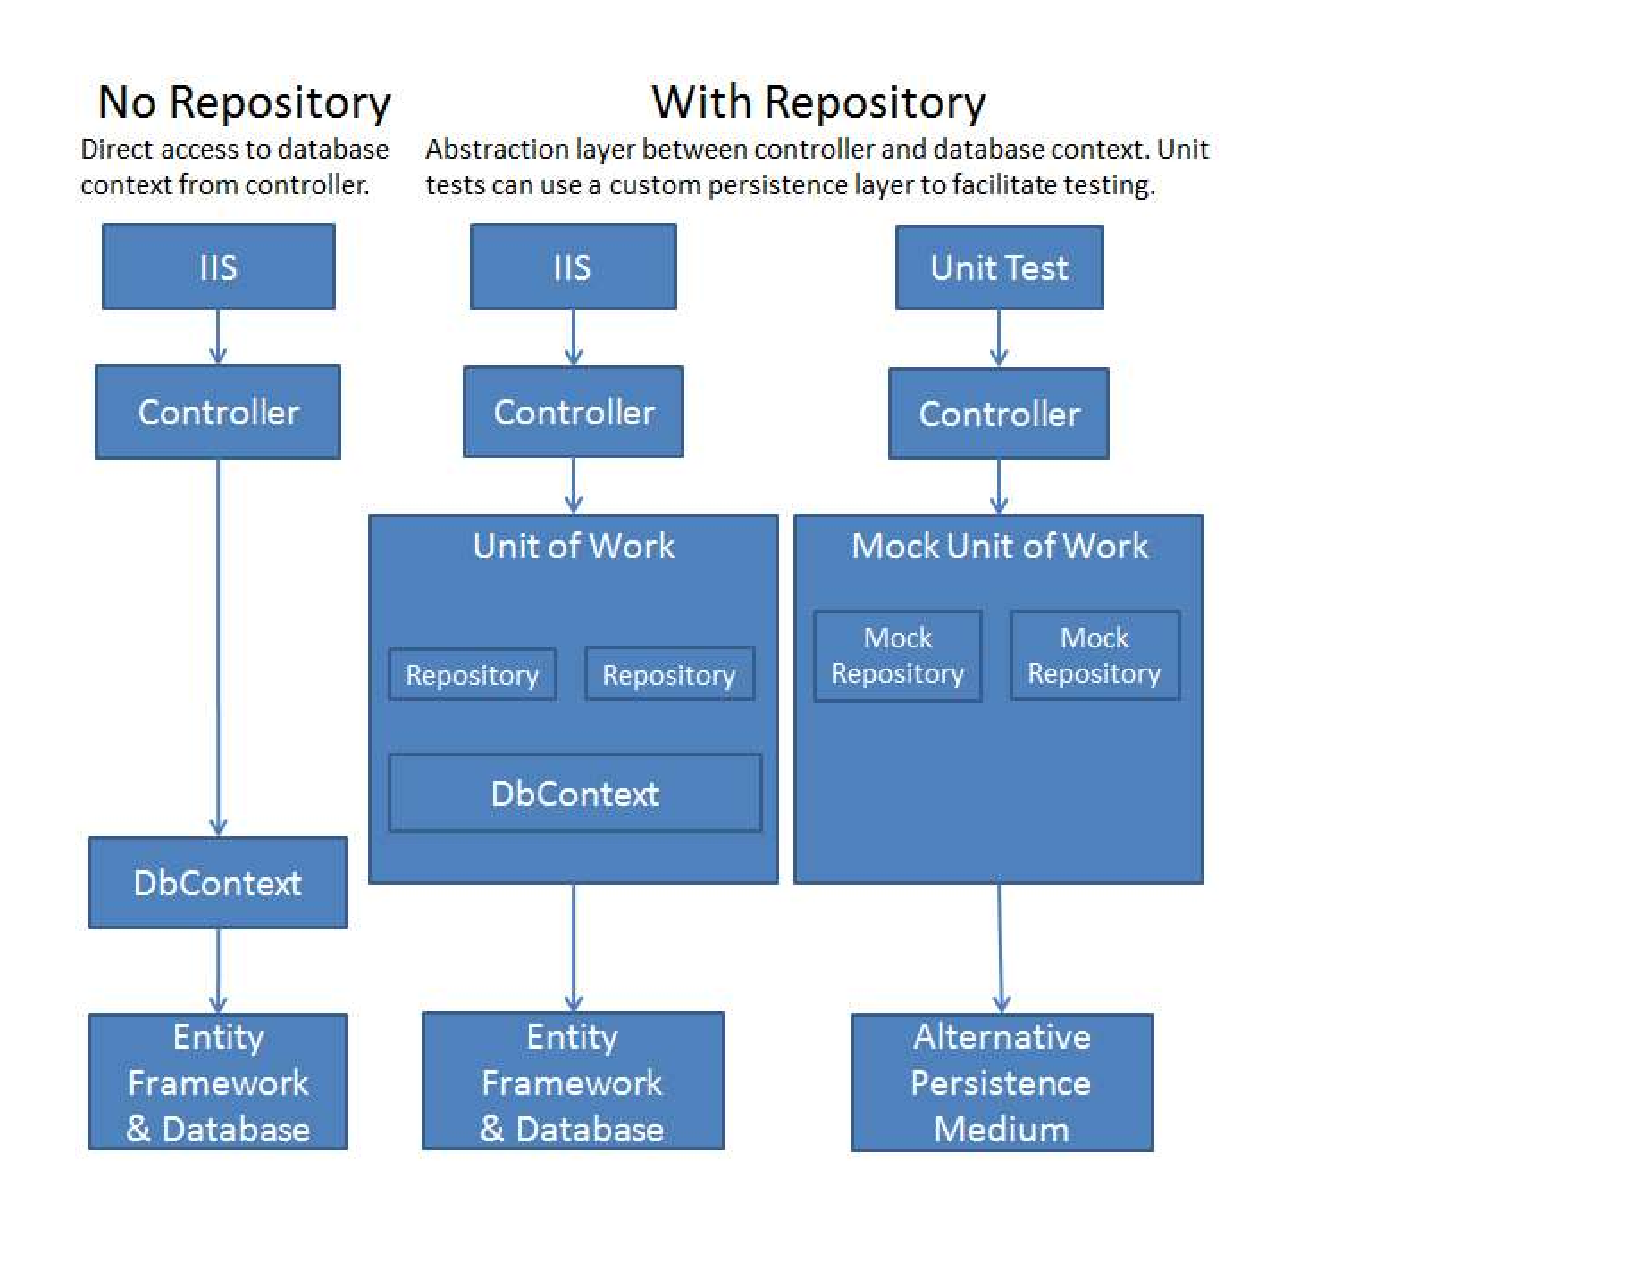
\includegraphics
	[width=165mm]{figures/RepsitoryTestFigure.PDF}
	\caption{Unit test med UnitOfWorkMock}
	\label{fig:UnitOfWorkMock}
\end{figure}